\subsection{Results on Effectiveness}
\label{effectiveness}

We now study the effectiveness of ACQ, and compare it with existing CD and CS methods. We then discuss a case study.

\subsubsection{ACQ Effectiveness}
\label{metric}

We first define two measures, namely CMF and CPJ, for evaluating the keyword cohesiveness of the communities.
Let $C(q)$=$\{C_1$, $C_2, \cdots$, $C_{\mathcal{L}}\}$ be the set of $\mathcal L$ communities returned by an algorithm for a query vertex $q \in V$ (Note that $S$=$W(q)$).

$\bullet$ {\bf Community member frequency (CMF)}:  this is inspired by the classical document frequency
measure. Consider a keyword $x$ of $q$'s keyword set $W(q)$. If $x$ appears in most of the vertices (or members) of  a community $C_i$, then we regard $C_i$ to be highly cohesive. The CMF uses the occurrence frequencies of $q$'s keywords in $C_i$ to determine the degree of cohesiveness. Let $f_{i,h}$ be the number of vertices of $C_i$ whose keyword sets contain the $h$-th keyword of $W(q)$. Then, $\frac{f_{i,h}}{|C_i|}$ is the relative occurrence frequency of this keyword in $C_i$. The CMF is the average of this value over all keywords in
$W(q)$, and all communities in $C(q)$:
\begin{equation}
\begin{small}
  \label{eq:amf}
    CMF(C(q)) = \frac{1}{{{\cal L} \cdot \left| {W(q)} \right|}}\sum\limits_{i = 1}^{\cal L} {\sum\limits_{h=1}^{\left| {W(q)} \right|} {\frac{{{f_{i,h}}}}{{|{C_i}|}}} }
 \end{small}
\end{equation}
Notice that $CMF(C(q))$ ranges from 0 to 1. The higher its value, the more cohesive is a community.

$\bullet$ {\bf Community pair-wise Jaccard (CPJ)}: this is based on the similarity between the keyword sets of any pair of vertices of community $C_i$. We adopt the Jaccard similarity, which is commonly used in the IR literature. Let $C_{i,j}$ be the $j$-th vertex of $C_i$.  The CPJ is then the average similarity over all pairs of vertices of $C_i$, and all communities of $C(q)$:
\begin{equation}
  \small
  \label{eq:apj}
    CPJ(C(q))=\frac{1}{{\cal L}}\sum\limits_{i = 1}^{\cal L} {\left[ {\frac{1}{{|{C_i}{|^2}}}\sum\limits_{j = 1}^{|{C_i}|} {\sum\limits_{k = 1}^{|{C_i}|} {\frac{{\left| {W({C_{i,j}}) \cap W({C_{i,k}})} \right|}}{{\left| {W({C_{i,j}}) \cup W({C_{i,k}})} \right|}}} } } \right]}
\end{equation}
The $CPJ(C(q))$ value has a range of 0 and 1. A higher value of $CPJ(C(q))$ implies better cohesiveness.

{\bf 1. Effect of common keywords.} We examine the impact of the AC-label length
(i.e., the number of keywords shared by all the vertices of the AC) on keyword cohesiveness.
We collect ACs containing one to five keywords, and then group the ACs according to their AC-label lengths. The average CMF and CPJ value of each group is shown in Figure~\ref{fig:measure-share}. For all the datasets, when the AC-label lengths increase, both CMJ and CPJ value rises. This justifies the use of the maximal AC-label length as the criterion of returning an AC in our ACQ Problem.

\begin{figure}[ht]
    \centering
    \mbox{
        \subfigure[CMF]{
            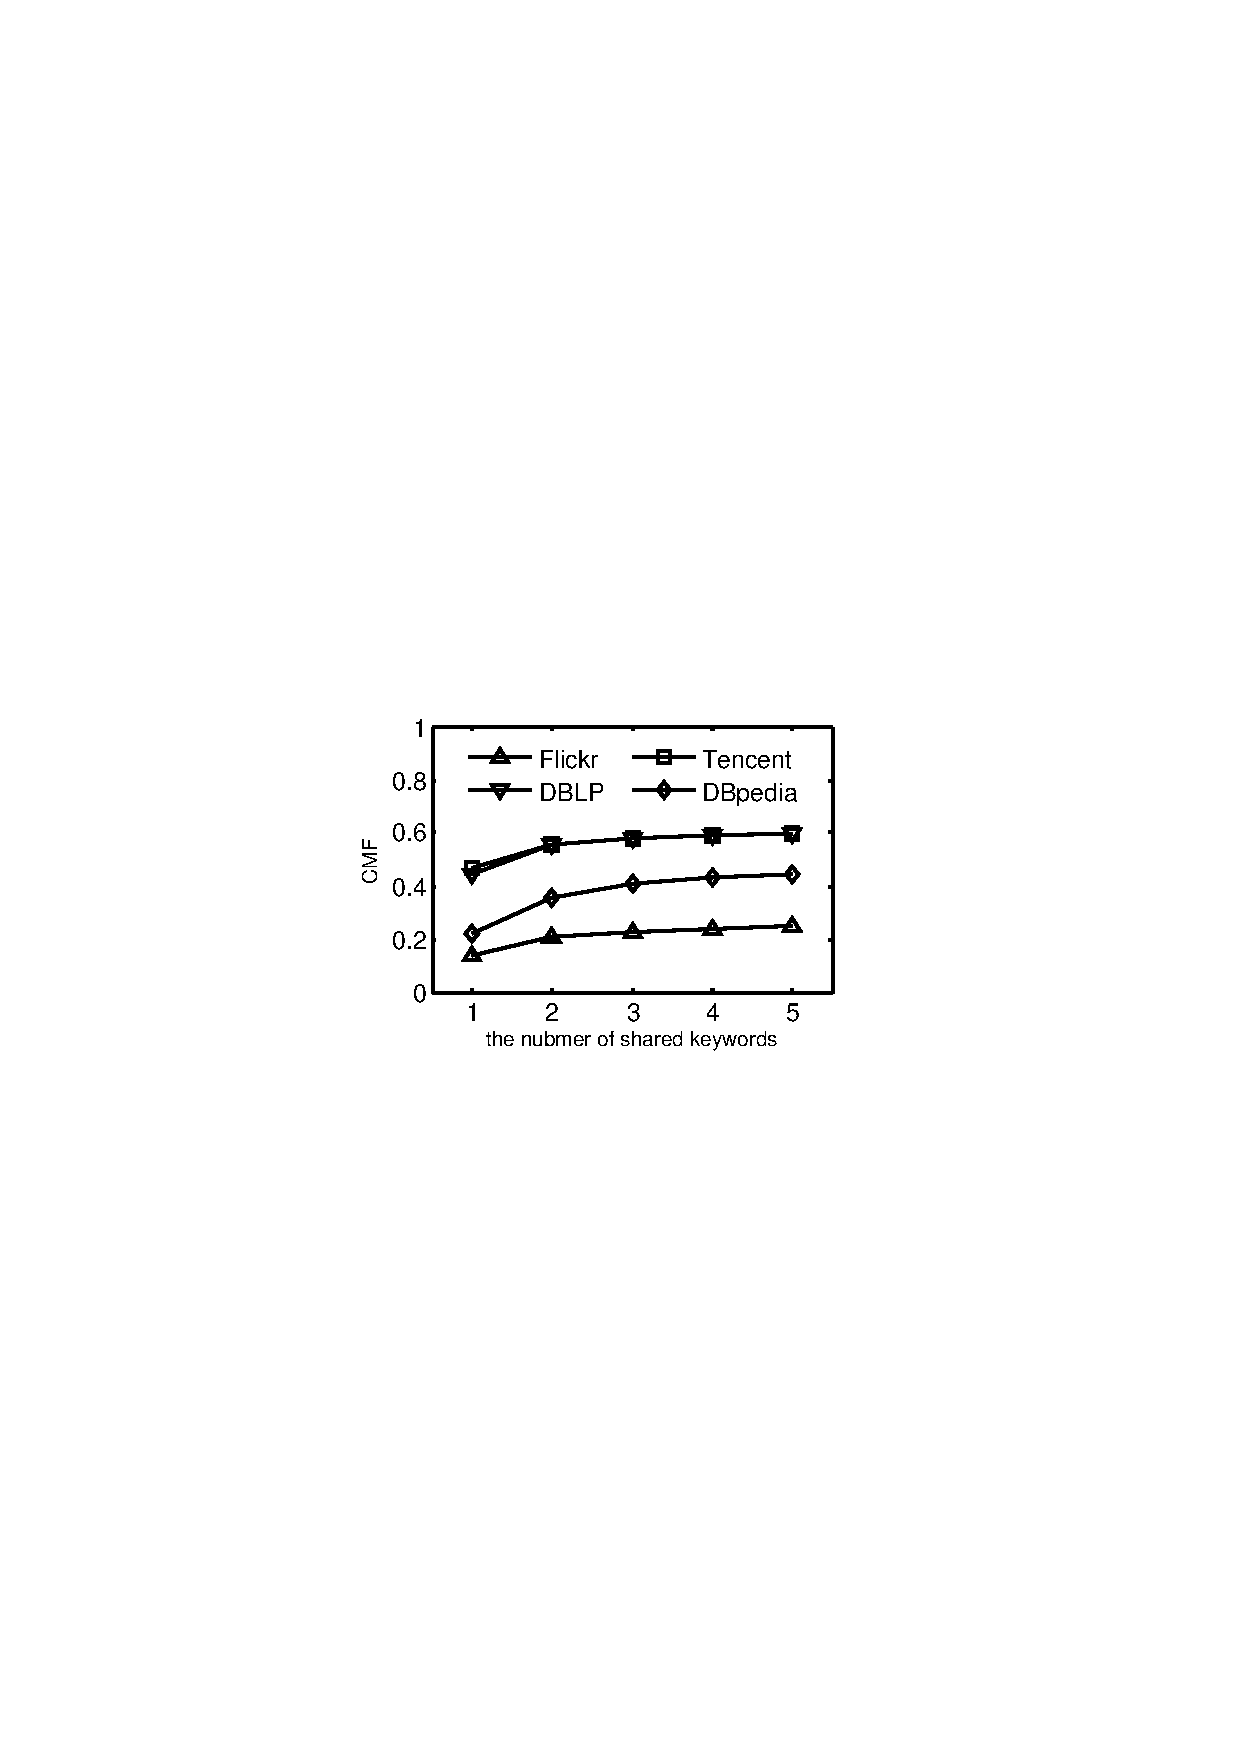
\includegraphics[width=.40\columnwidth]{figures/cmf-share}
            \label{fig:aqj}
        }
        \hspace{2ex}
        \subfigure[CPJ]{
            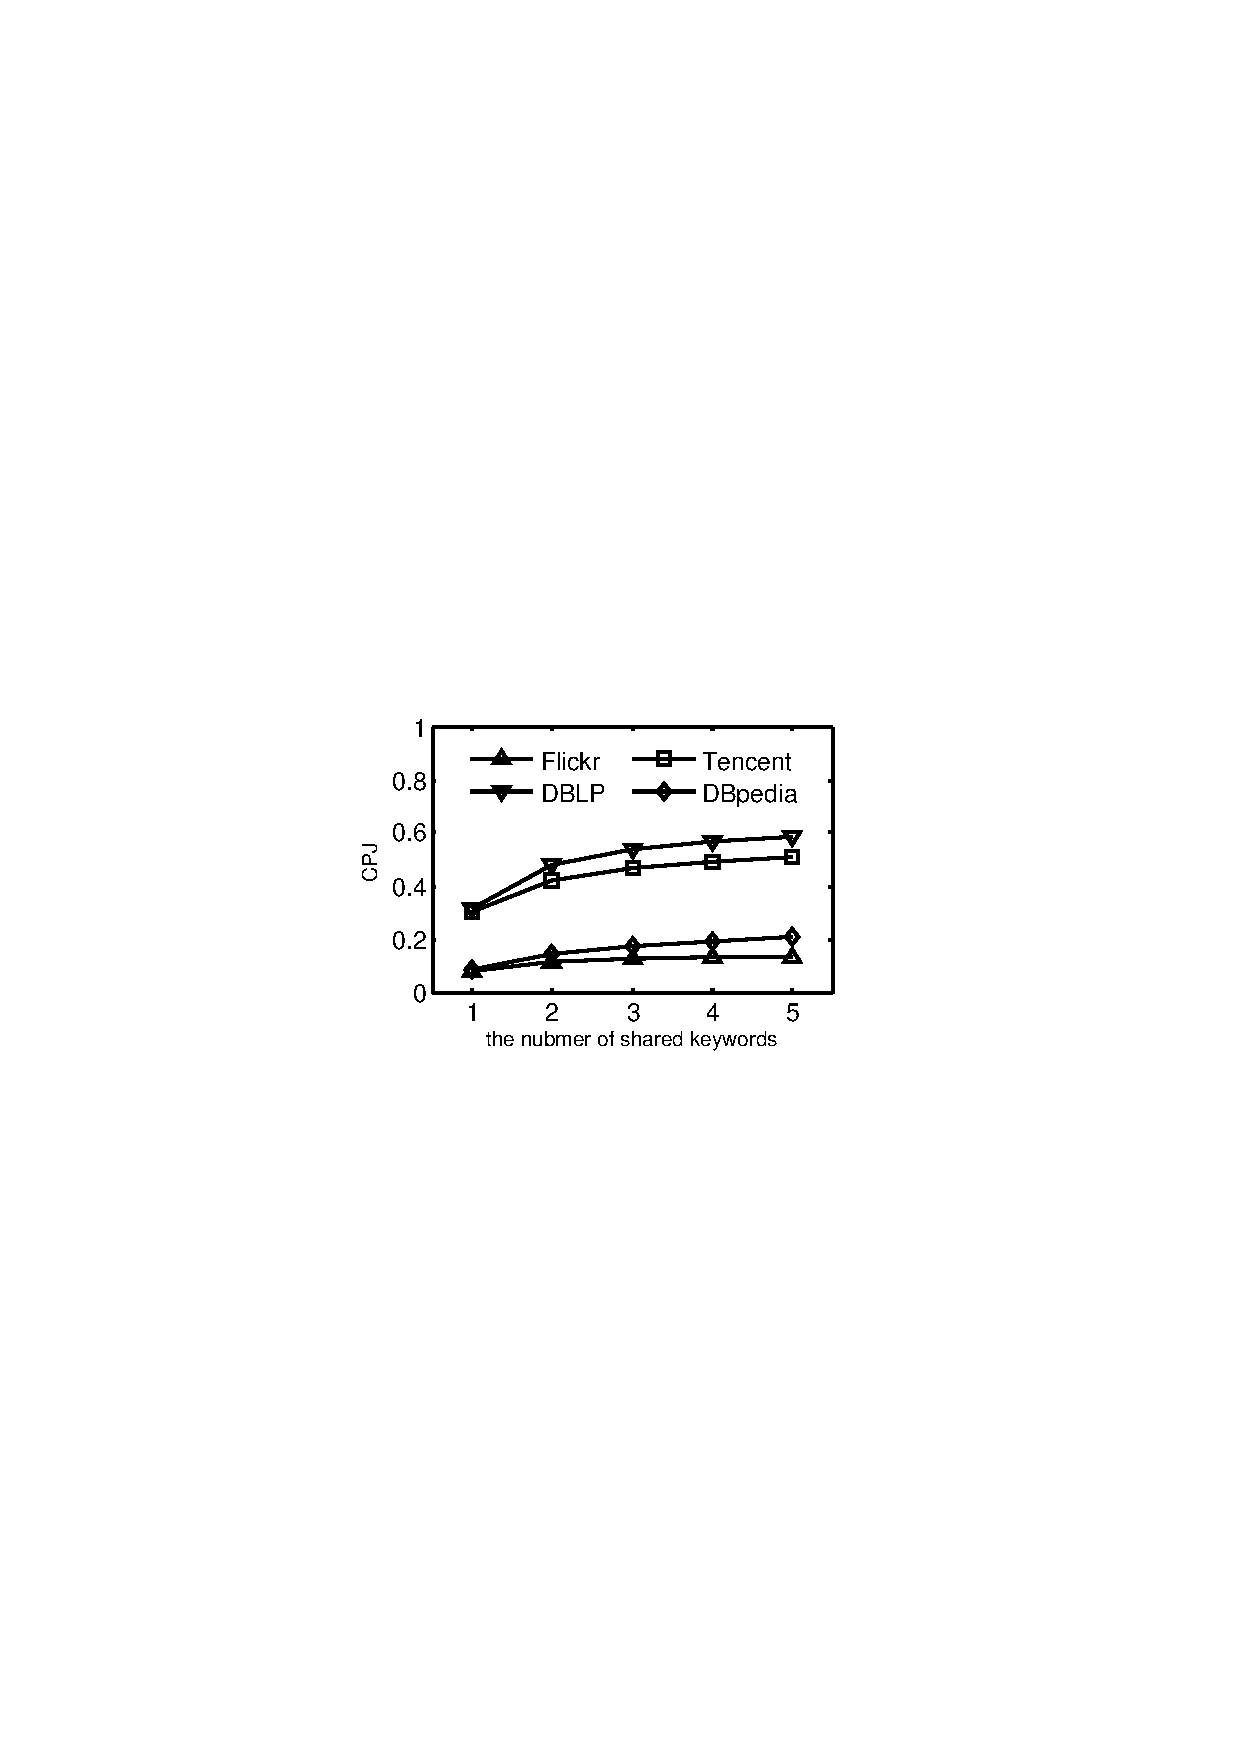
\includegraphics[width=.40\columnwidth]{figures/cpj-share}
            \label{fig:apj}
        }
    }
    \caption{AC-label length.}\label{fig:measure-share}
\end{figure}


{\bf 2. Comparison with existing CD methods}
As mentioned ahead, the existing CD methods for attributed graph can be adapted for community search. We choose to adapt {\tt CODICIL}~\cite{attr-www2013} for comparison. The main reasons are: (1) it has been tested on the ever reported largest attributed graph (vertex number:3.6M); (2) it identifies communities of comparable or superior quality than those of many existing methods like~\cite{attr-topic-kdd2008,attr-kdd2009}; and (3) it runs faster than many existing methods. Since {\tt CODICIL} needs users to specify the number of clusters expected, we set the numbers as 1K, 5K, 10K, 50K and 100K. The corresponding adapted algorithms are named as {\tt Cod1K}, $\cdots$, {\tt Cod100K} respectively. Other parameter settings are the same as those in~\cite{attr-www2013}. We first run these algorithms offline to obtain all the communities. Given a query vertex $q$, they return communities containing $q$ as the results.

We consider both keyword and structure for evaluating community quality.
(1) \emph{Keyword:} Figures~\ref{fig:detection-comp}(a) and (b) show that {\tt ACQ} (implemented by {\tt Dec}) always performs the best, in terms of CMF and CPJ.
(2) \emph{Structure:} As {\tt CODICIL} has no guarantee on vertices' minimum degrees, it is unfair to compare them using this metric. We intuitively compare their structure cohesiveness by reporting the average degree of the vertices in the communities and the percentage of vertices having degrees of 6 or more. When the number of clusters in {\tt CODICIL} is too large or too small, the structure cohesiveness becomes weak, as shown in Figures~\ref{fig:detection-comp}(c) and (d). {\tt ACQ} always performs better than {\tt CODICIL}, even when its number of cluster is well set (e.g., {\tt Cod10K} and {\tt Cod50K} on DBLP dataset).

\begin{figure}[]
\centering
    \begin{tabular}{c c}
        \begin{minipage}{3.36cm}
	        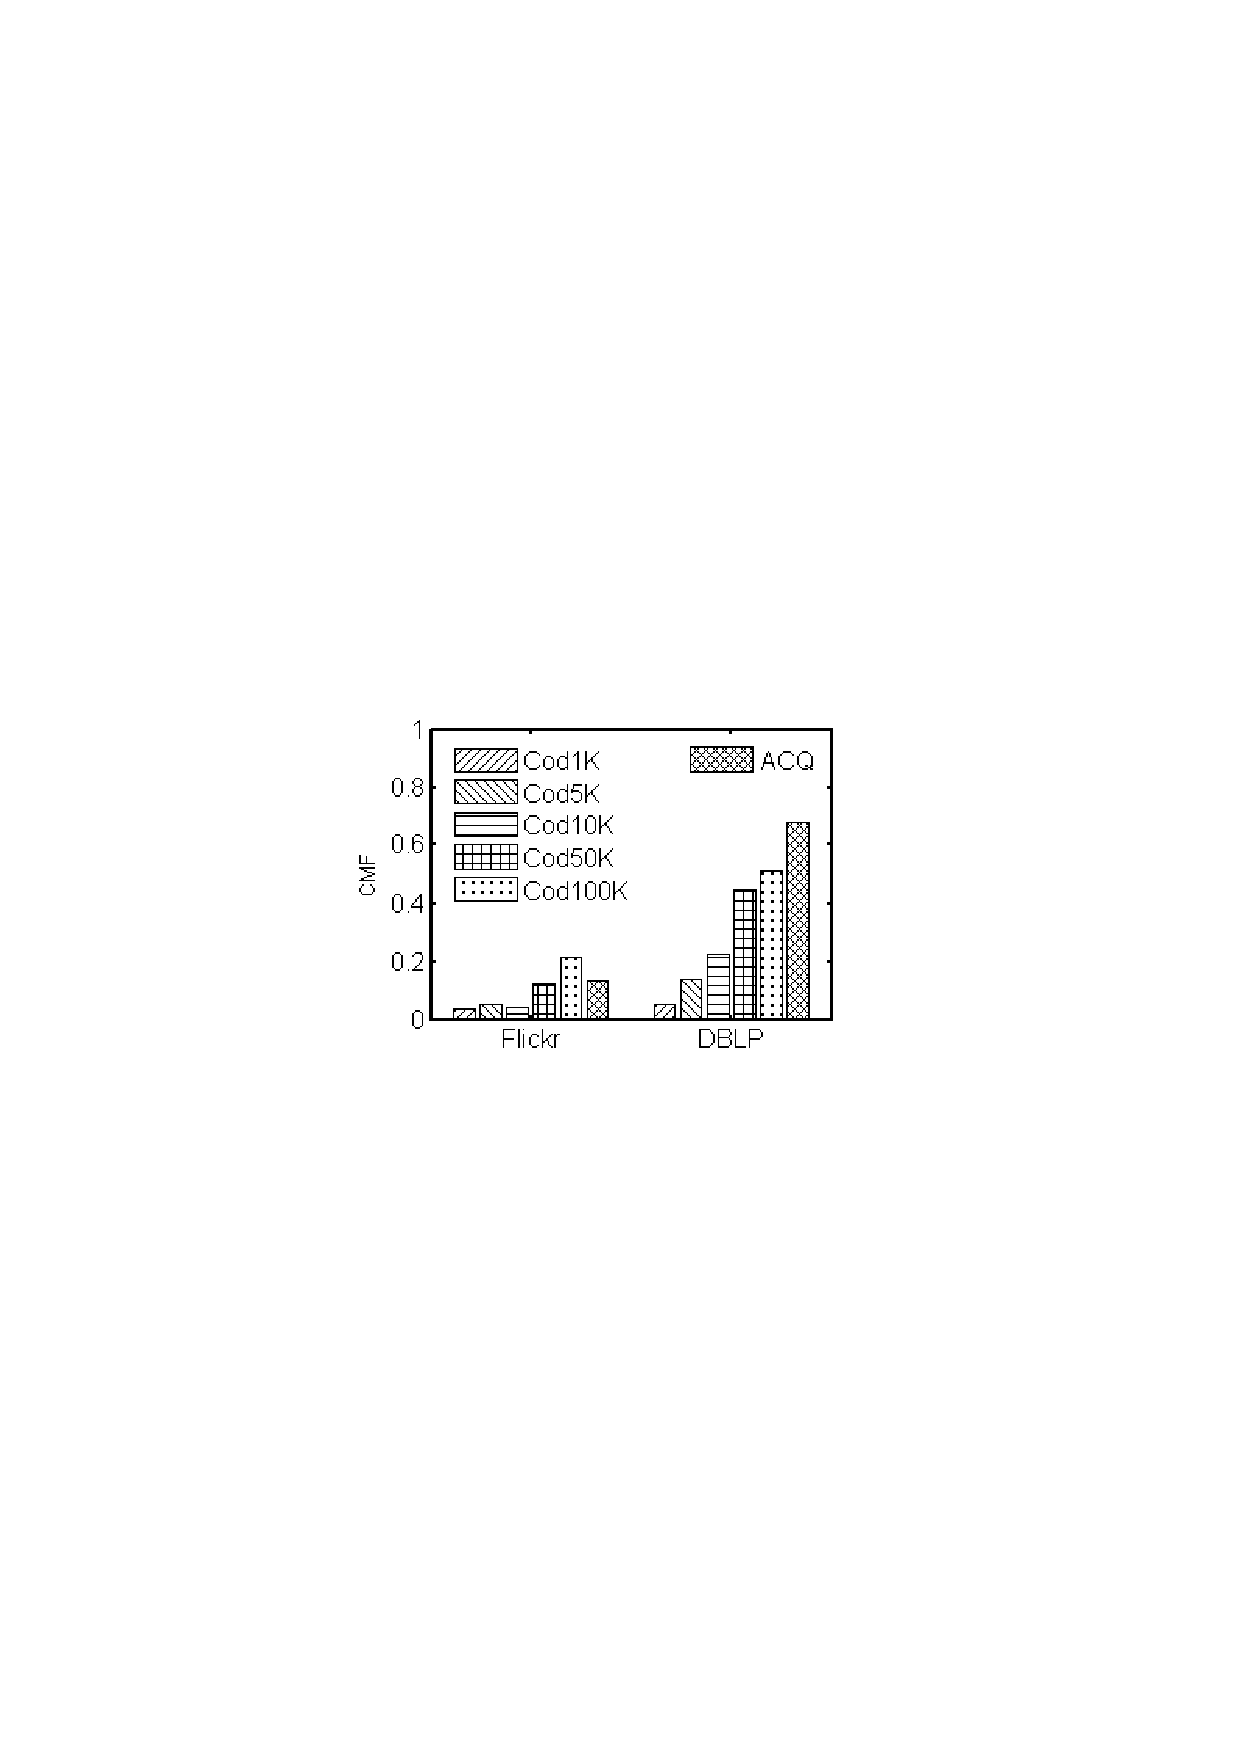
\includegraphics[width=3.35cm]{figures/cmfCOD}
        \end{minipage}
        &
        \begin{minipage}{3.36cm}
	     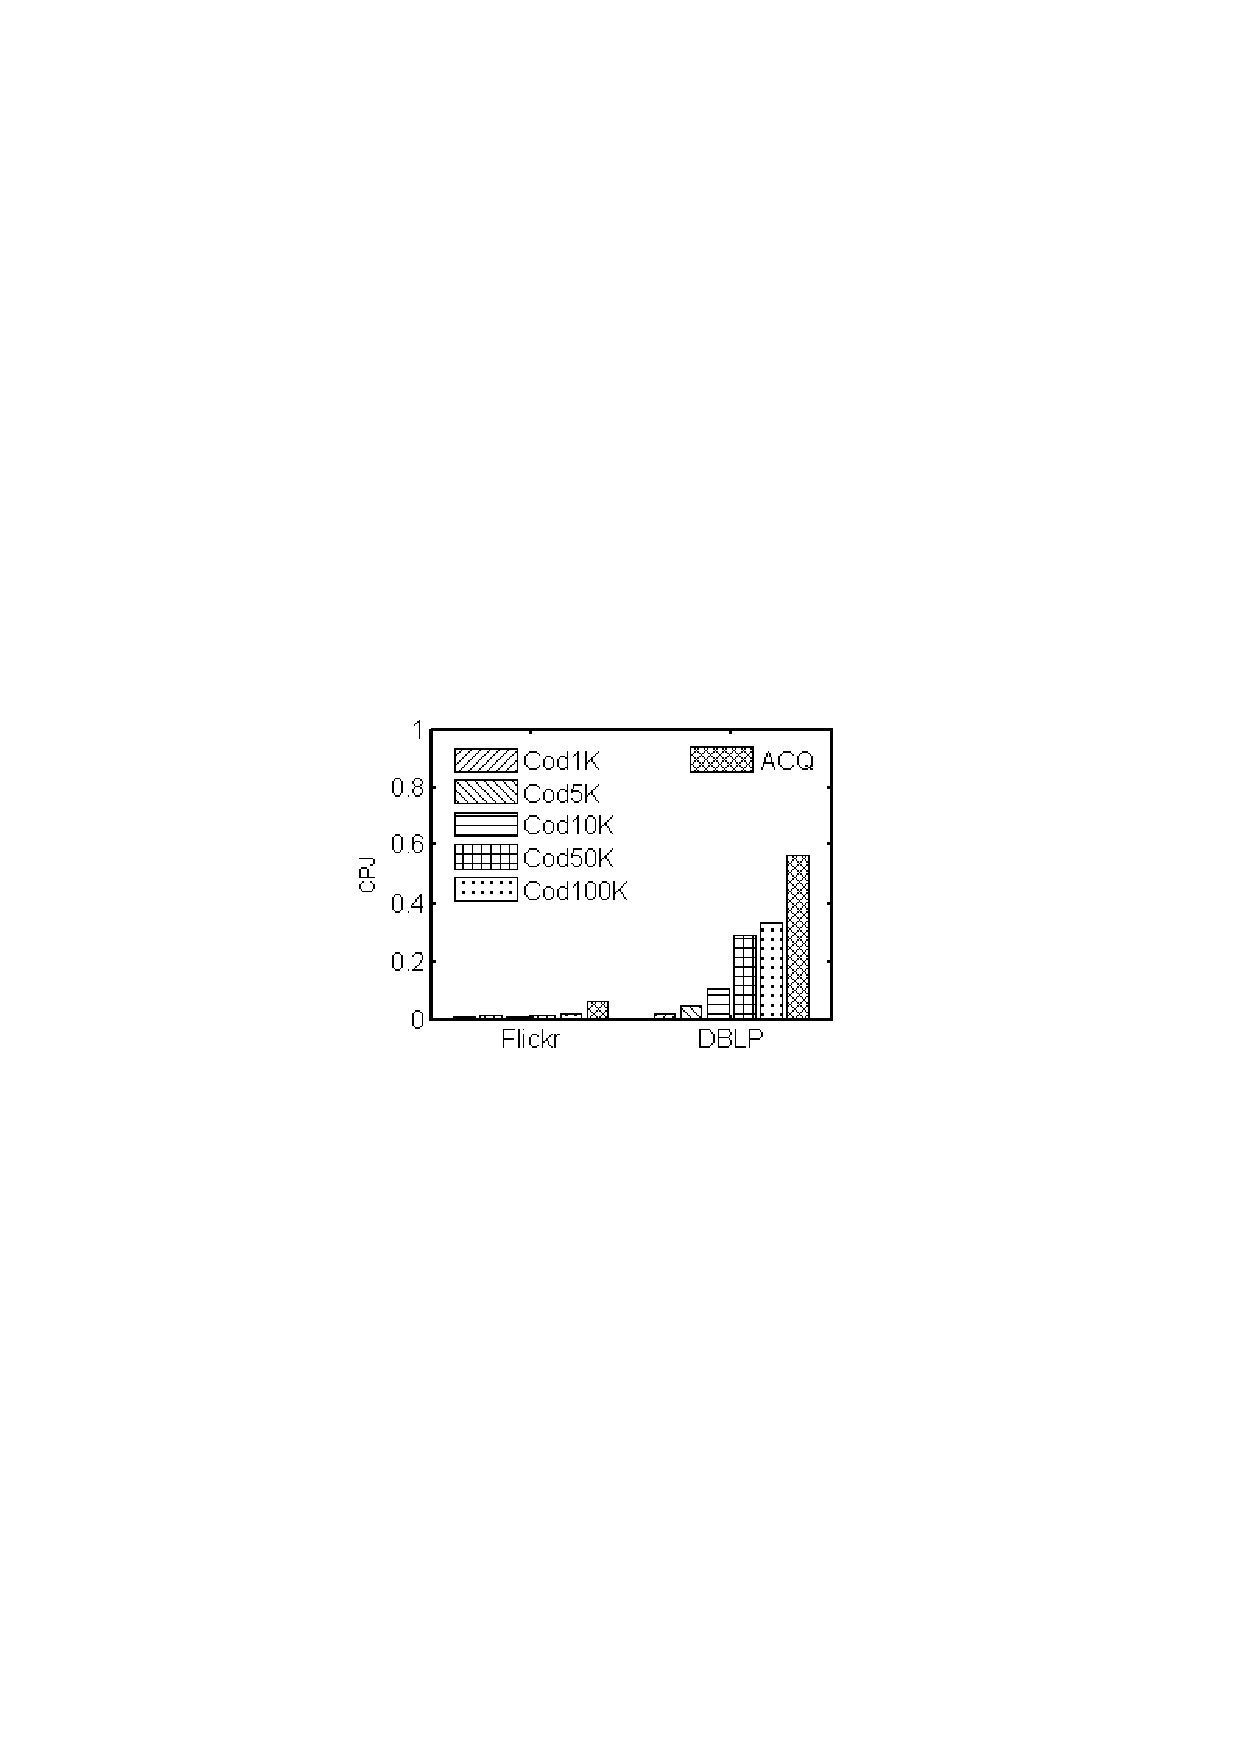
\includegraphics[width=3.35cm]{figures/cpjCOD}
         \end{minipage}
         \\
         \small (a) Keyword (CMF)
         &
         \small (b) Keyword (CPJ)
         \\

        \begin{minipage}{3.36cm}
	       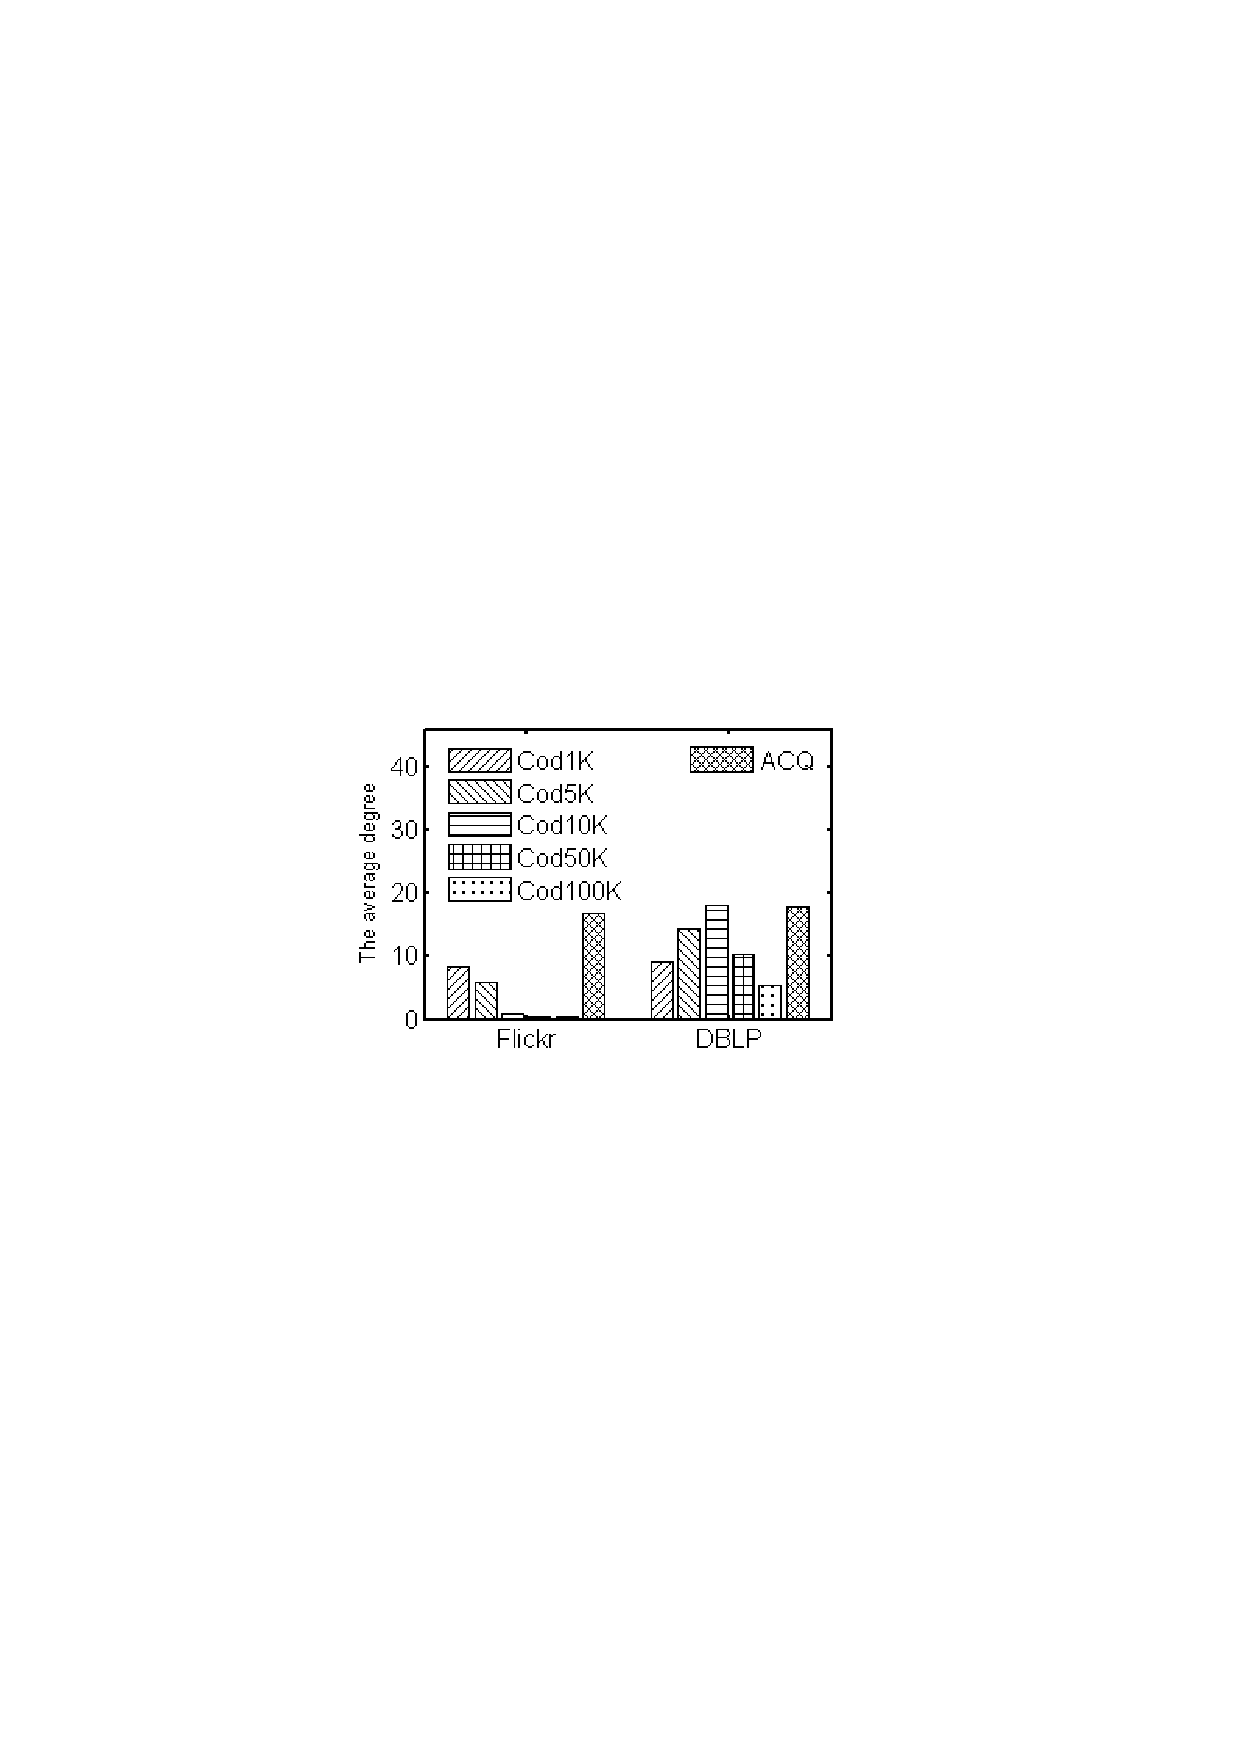
\includegraphics[width=3.35cm]{figures/avgDegCOD}
        \end{minipage}
        &
        \begin{minipage}{3.36cm}
	       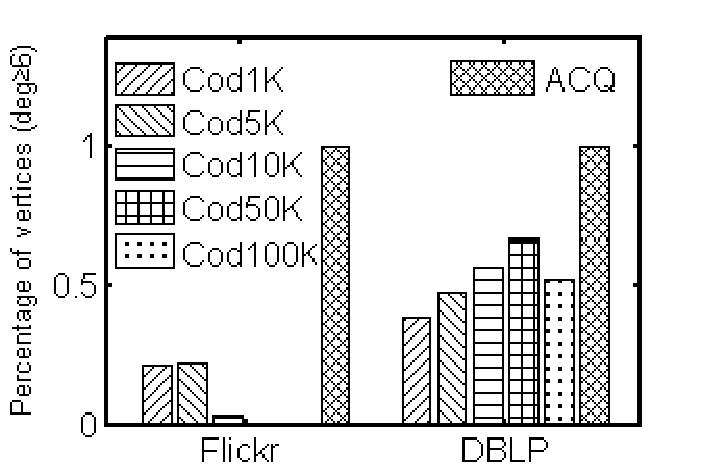
\includegraphics[width=3.35cm]{figures/deg6COD}
        \end{minipage}
        \\
        \small (c) Structure (Avg. degree)
        &
        \small (d) Structure (degree $\geq$ 6)
    \end{tabular}
    \caption{Comparing with community detection method.}
    \label{fig:detection-comp}
\end{figure}


{\bf 3. Comparison with existing CS methods.}
The existing methods mainly focus on non-attributed graphs. We implement two state-of-the-art methods:
{\tt Global}~\cite{KDD2010} and {\tt Local} \cite{local2014}. Both of them use the metric minimum degree, we thus focus on the keyword cohesiveness. Figure~\ref{fig:search-comp} shows the CMF and CPJ values on four datasets. We can see that the keyword cohesiveness of {\tt ACQ} is superior to both {\tt Global} and {\tt Local}, because {\tt ACQ} considers vertex keywords, while {\tt Global} and {\tt Local} do not.

\begin{figure}[ht]
    \centering
    \mbox{
        \subfigure[CMF]{
            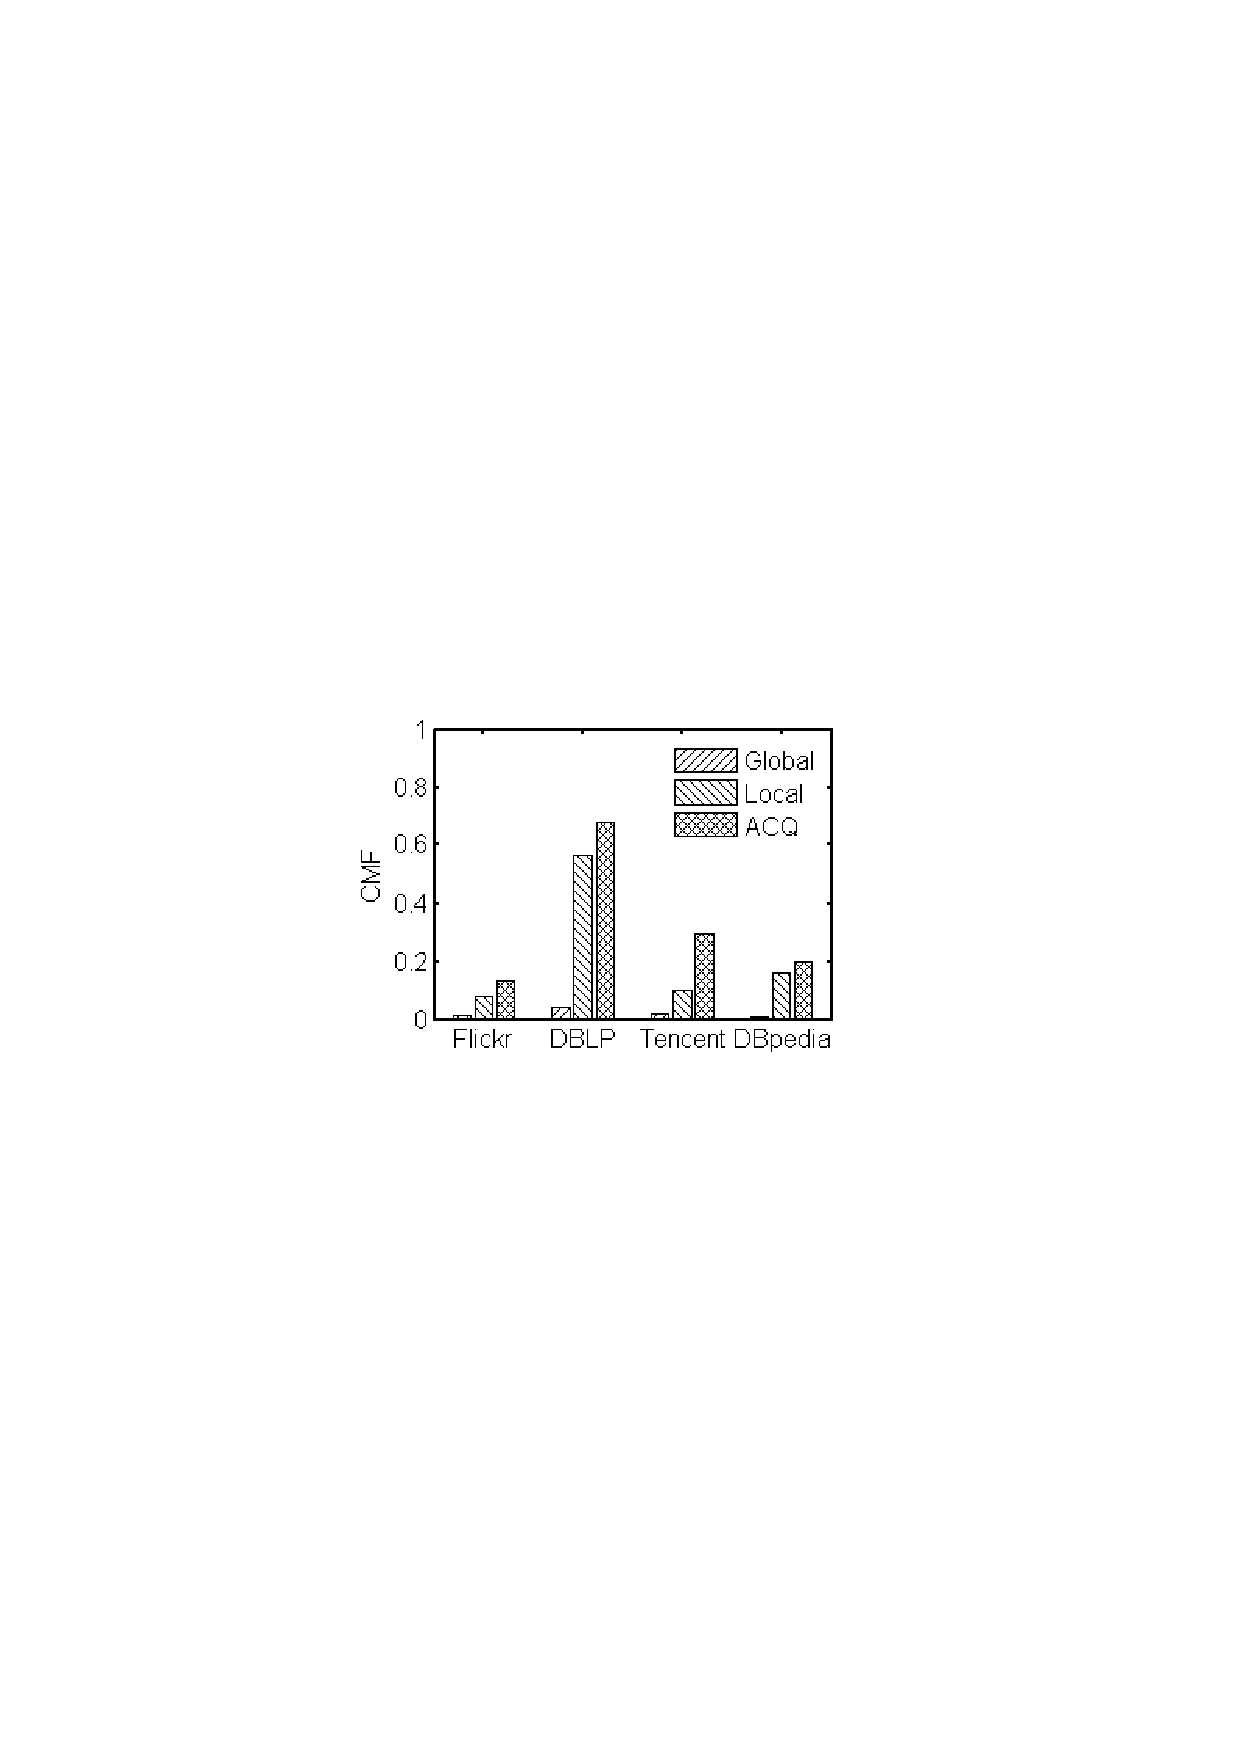
\includegraphics[width=.40\columnwidth]{figures/cmf}
            \label{fig:cmf}
        }
        \hspace{2ex}
        \subfigure[CPJ]{
            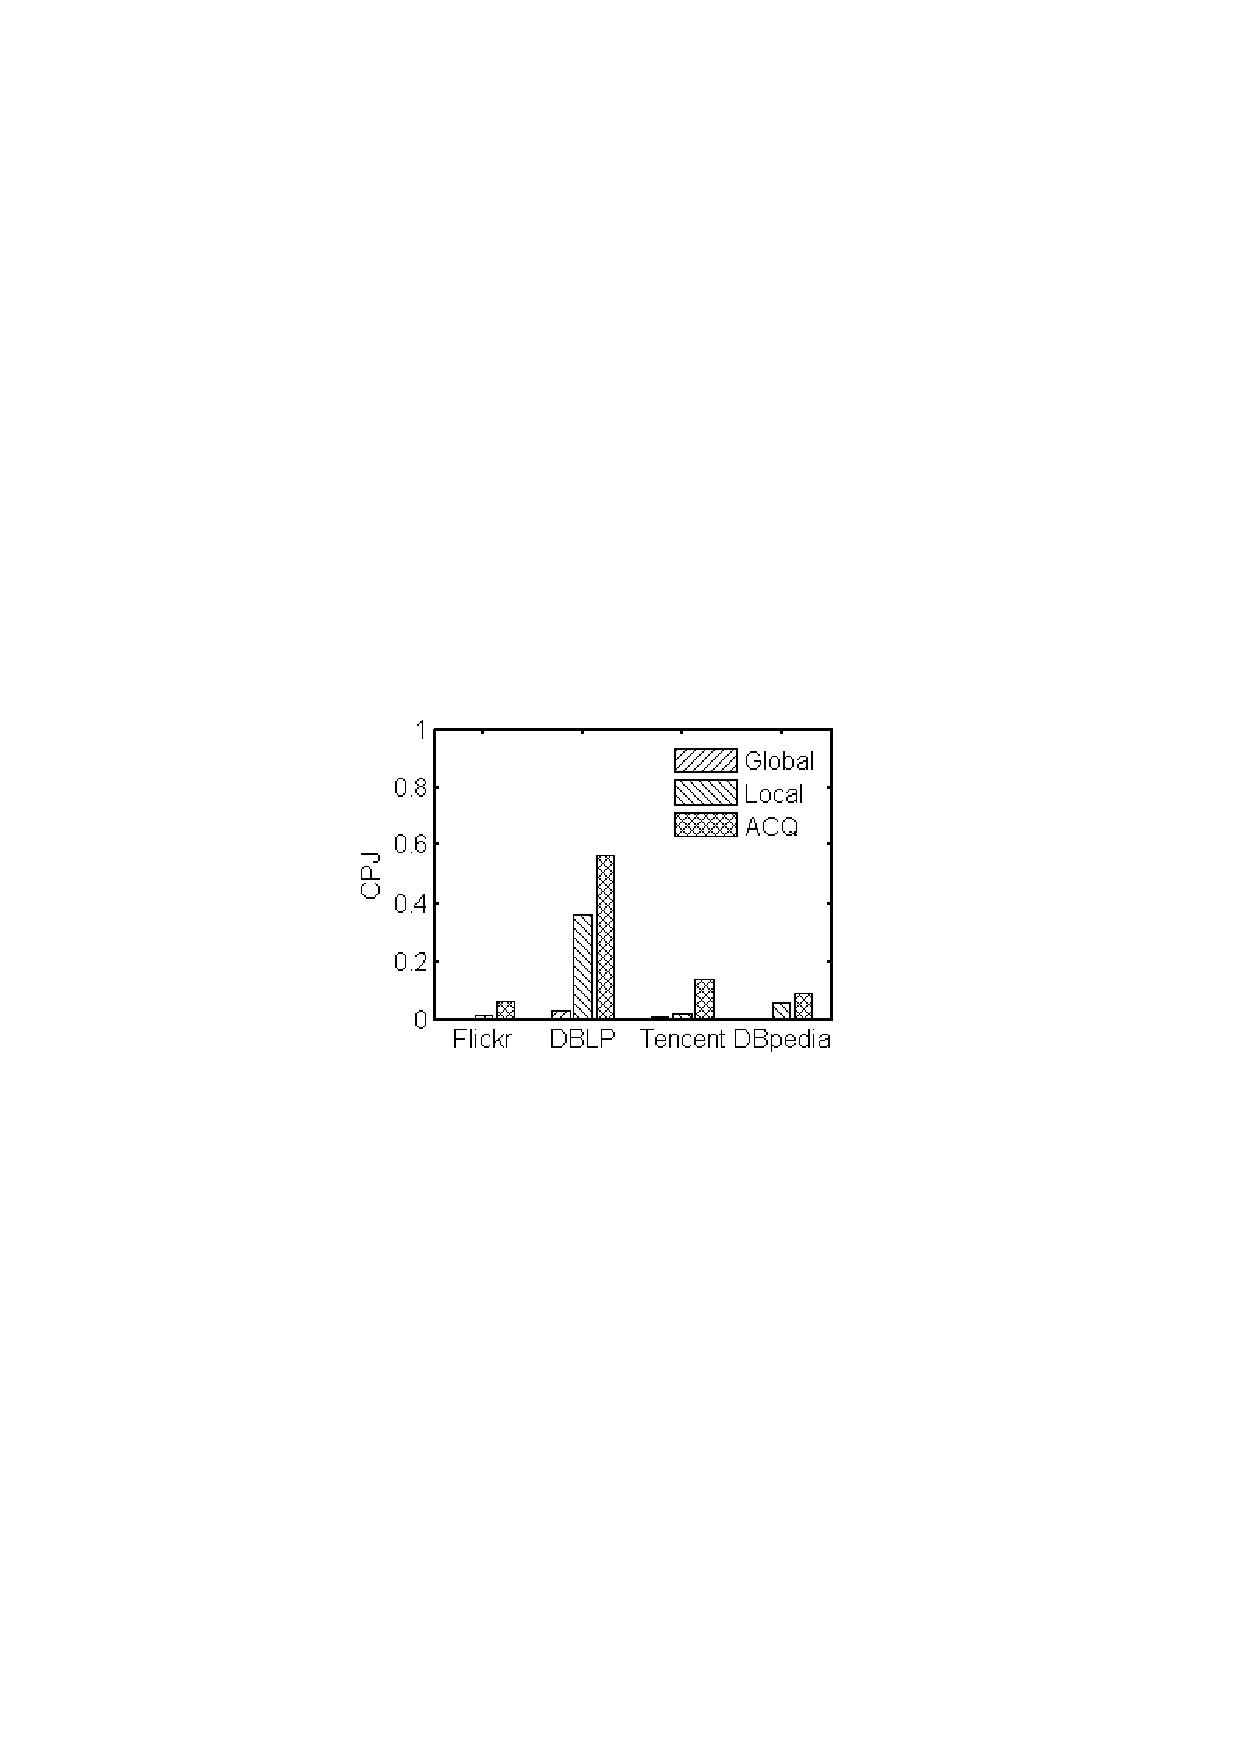
\includegraphics[width=.40\columnwidth]{figures/cpj}
            \label{fig:cpf}
        }
    }
    \caption{Comparing with community search methods.}
    \label{fig:search-comp}
\end{figure}

\subsubsection{A Case Study}
\label{caseStudy}

We next perform a case study on the DBLP dataset, in which we consider two renowned researchers in database and data mining: Jim Gray and Jiawei Han. We use $k=4$ here. We use {\tt Cod50K} to represent {\tt CODICIL} for further analysis.
We mainly consider the input query keyword set $S$, keywords and sizes of communities.

{\bf 1. Effect of $S$.} Figure~\ref{fig:jiawei} shows two ACs of Jiawei (AC-labels are shown in the captions),
where the query keyword set $S$ are set as $\{$analysis, mine, data, information, network$\}$ and $\{$mine, data, pattern, database$\}$ respectively. These two groups of Jiawei's collaborators are involved in graph analysis (Figure~\ref{fig:jiawei1}) and pattern mining (Figure~\ref{fig:jiawei2}). Although these researchers all have close co-author relationship with Jiawei, the use of the input keyword set $S$ enables the identification of communities with different research themes.
For Jim, we can obtain similar results as discussed in Section~\ref{intro} (Figure~\ref{fig:jim}).
While for {\tt CODICIL}, it is not clear how to consider the keyword set $S$, and we thus do not show the results.

\begin{figure}[ht]
    \centering
    \mbox{
        \subfigure[$\{$analysis, data, information, network$\}$]{
            
\includegraphics[width=.40\columnwidth]{figures/jiawei1}
            \label{fig:jiawei1}
        }
        \hspace{2ex}
        \subfigure[$\{$mine, data, pattern, database$\}$]{
            
\includegraphics[width=.40\columnwidth]{figures/jiawei2}
            \label{fig:jiawei2}
        }
    }
    \caption{Jiawei Han's ACs.}
    \label{fig:jiawei}
\end{figure}

\begin{figure}[h]
    \centering
    \mbox{
        \subfigure[Jim Gray]{
            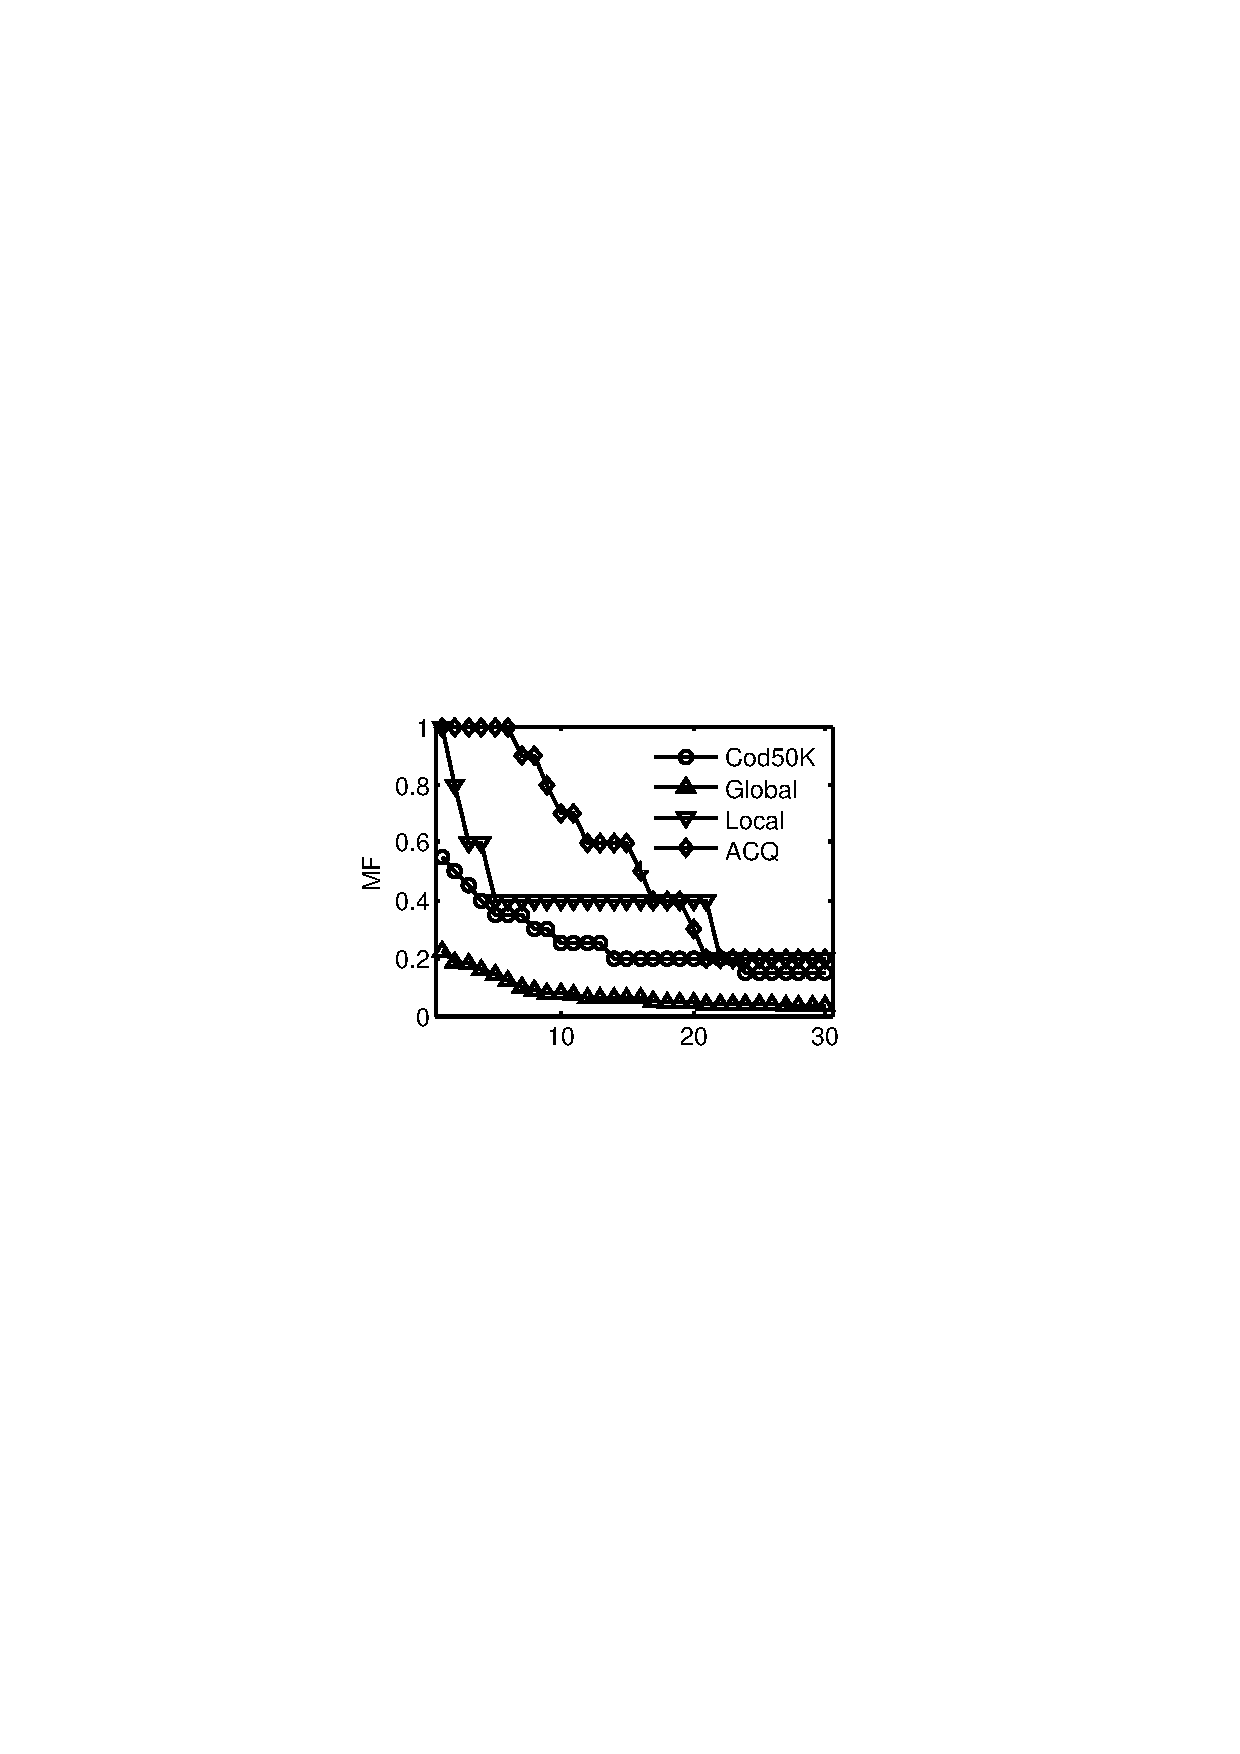
\includegraphics[width=.40\columnwidth]{figures/jim-mf}
            \label{fig:jimFreq30}
        }
        \hspace{2ex}
        \subfigure[Jiawei Han]{
            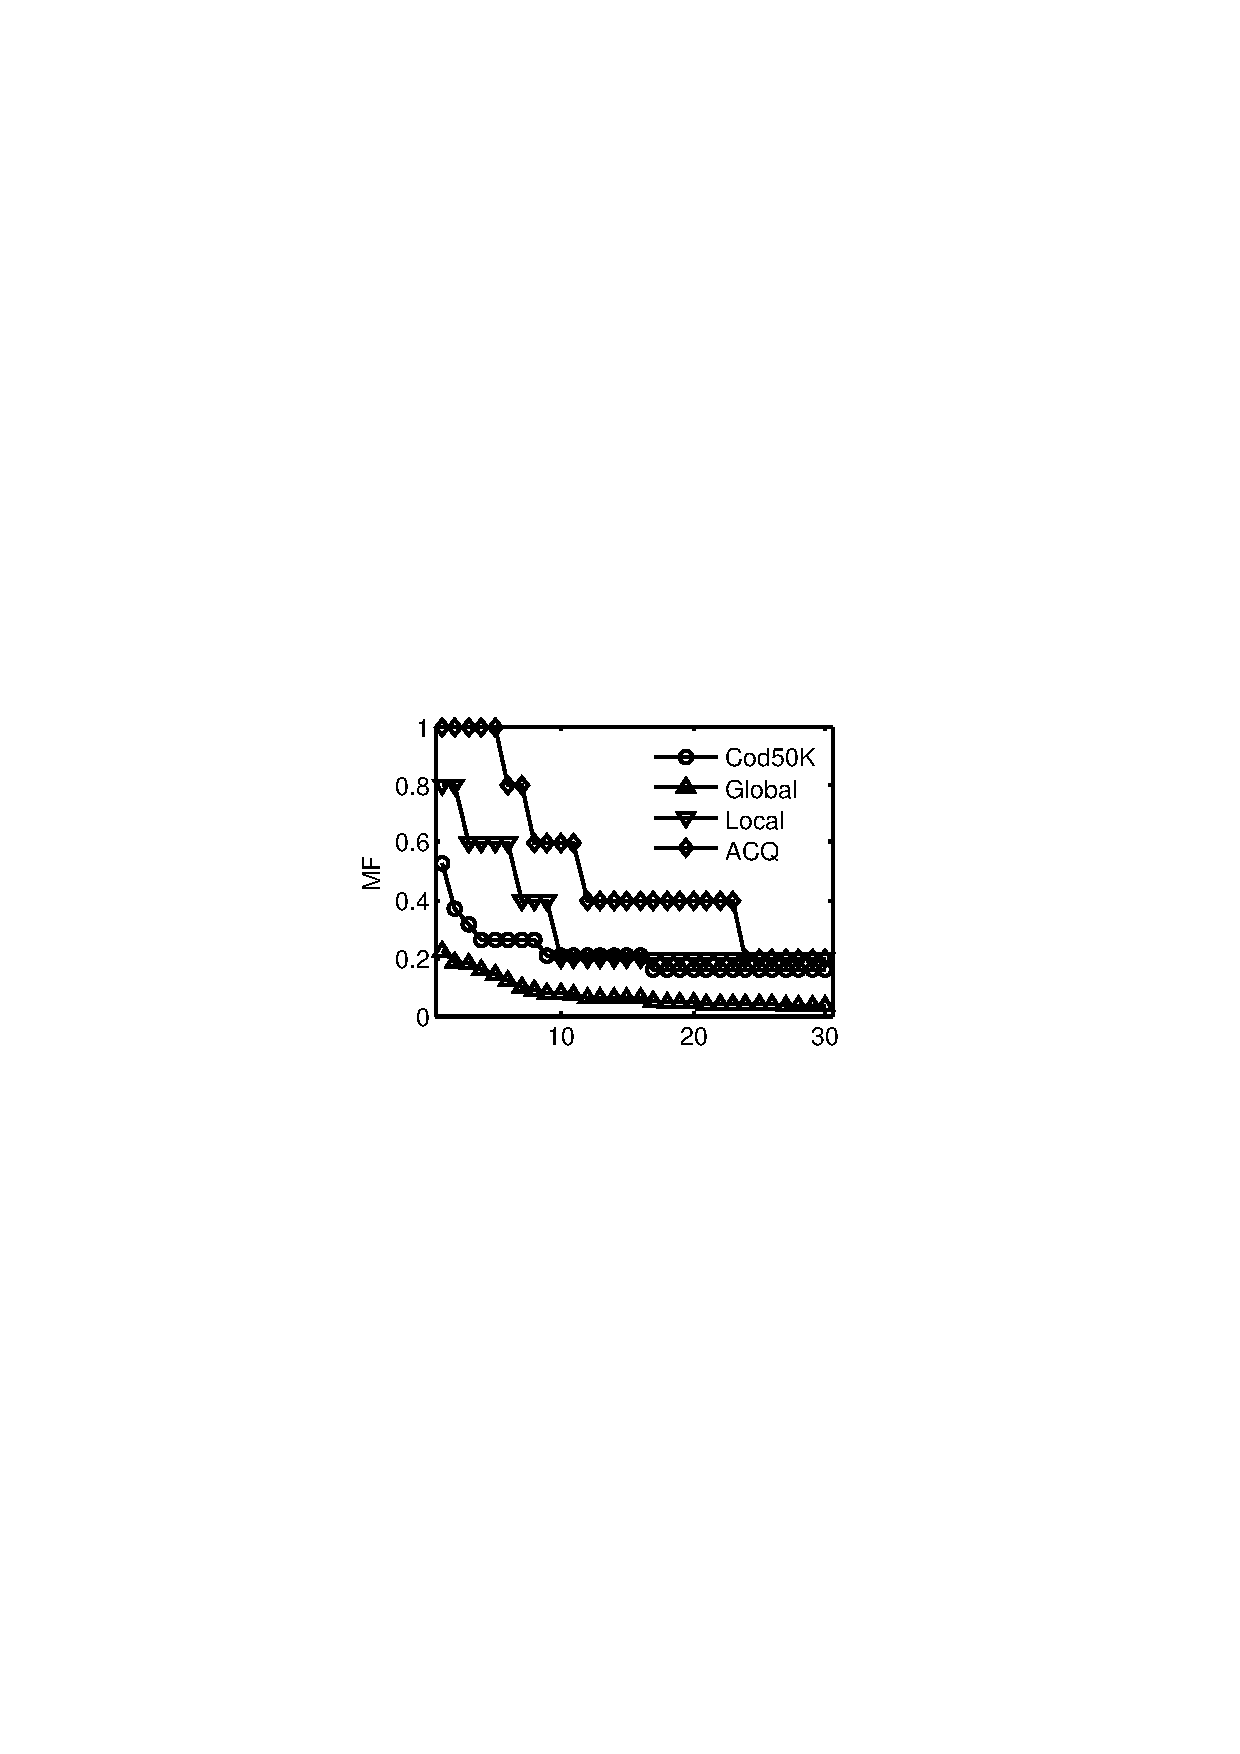
\includegraphics[width=.40\columnwidth]{figures/jiawei-mf}
            \label{fig:jiaweiFreq30}
        }
    }
    \caption{Frequency distribution of keywords.}\label{fig:freq50}
\end{figure}

\vspace{-0.2cm}
\begin{table}[h]
  \centering \footnotesize \caption {\# distinct keywords of communities.}
  \label{tab:kws}
  \begin{tabular}{c|c|c|c|c}
     \hline
          \bf{Researcher}            & {\tt Cod50K} &  \bf{{\tt Global}} & {\tt Local} & {\tt ACQ}\\
     \hline\hline
          Jim Gray   &     134       & 139,881      &     60     &    44    \\
     \hline
          Jiawei Han &     140       & 139,881      &     58     &    54\\
     \hline
  \end{tabular}
\end{table}

{\bf 2. Keyword analysis.} We analyze the frequency distribution of keywords in their communities.
Specifically, given a keyword $w_h$, we define the member frequency (MF) of $w_h$ as:
$MF({w_h}, C(q)) = \frac{1}{\mathcal{L}}\sum\limits_{i = 1}^\mathcal{L} {\frac{{{f_{i,h}}}}{{\left| {{C_i}} \right|}}}$.
The MF measures the occurrence of a keyword in $C(q)$. For each $C_q$ generated by an algorithm, we select 30 keywords with the highest MF values. We report the MF of each keyword in descending order of their MF values in Figure~\ref{fig:freq50}.
We see that {\tt ACQ} has the highest MF values for the top 20 keywords. Thus, the keywords associated with the communities generated by {\tt ACQ} tend to repeat among the community members.

The number of distinct keywords of {\tt ACQ} communities is also the fewest, as shown in Table~\ref{tab:kws}.
For example, the $k$-$\widehat{core}$ returned by {\tt Global} has over $139K$ distinct keywords,
about 2,300 times more than that returned by {\tt ACQ} (less than 60 keywords). While the semantics of the $k$-$\widehat{core}$ can be difficult to understand, the small number of distinct keywords of AC makes it easier to understand why the community is so formed. We further report the keywords with the 6 highest MF values in Jim and Jiawei's communities in Tables~\ref{tab:jim} and~\ref{tab:jiawei}. We can see that, words ``sloan'',  ``digital'', ``sky'', ``survey'', and ``sdss'' reflect that the community is likely about the SDSS project led by Jim. The top-6 keywords of Jiawei's AC are related to heterogenous networks. In contrast, the keywords of {\tt Global} and {\tt Local} tend to be less related to the query keyword set, and thus they cannot be used to characterize the communities specifically related to Jiawei.
Note that the top-6 keywords of {\tt Global} are the same for both Jim and Jiawei, as they are in the same $k$-$\widehat{core}$.
The overall results show that, {\tt ACQ} performs better than other methods.

\begin{table}[htp]
  \centering \footnotesize \caption {Top-6 keywords (Jim Gray).}
  \label{tab:jim}
  \begin{tabular}{c|l}
     \hline
          \bf{Algo.}   & \multicolumn{1}{c}{\textbf{Keywords}}\\
     \hline\hline
          {\tt Cod50K} & server, archive, sloan, digital, database\\
     \hline
          {\tt Global} & use, system, model, network, analysis, data\\
     \hline
          {\tt Local}  & database, system, multipetabyte, data, lsst, story\\
     \hline
          {\tt ACQ}    & sloan, digital, sky, data, sdss, server\\
     \hline
  \end{tabular}
\end{table}

\begin{table}[htp]
  \centering \footnotesize \caption {Top-6 keywords (Jiawei Han).}
  \label{tab:jiawei}
  \begin{tabular}{c|l}
     \hline
          \bf{Algo.}   & \multicolumn{1}{c}{\textbf{Keywords}}\\
     \hline\hline
          {\tt Cod50K} & information, mine, data, cube, text, network\\
     \hline
          {\tt Global} & use, system, model, network, analysis, data\\
     \hline
          {\tt Local}  & scalable, topical, text, phrase, corpus, mine\\
     \hline
          {\tt ACQ}    & mine, analysis, data, information, network, heterog\\
     \hline
  \end{tabular}
\end{table}



\textbf{3. Effect of $k$ on community size.}  We vary the value of $k$ and report the average size of communities in Figure~\ref{fig:size}. We can see that  the communities returned by {\tt Global} are extremely large (more than $10^5$), which can make them difficult for a query user to analyze. The community size of {\tt Local} increases sharply when $k$=8. In this situation, {\tt Local} returns the same community as {\tt Global}. The size of an AC is relatively insensitive to the change of $k$, as AC contains around a hundred vertices for a wide range of values of $k$.

\begin{figure}[ht]
    \centering
    \mbox{
        \subfigure[Jim Gray]{
            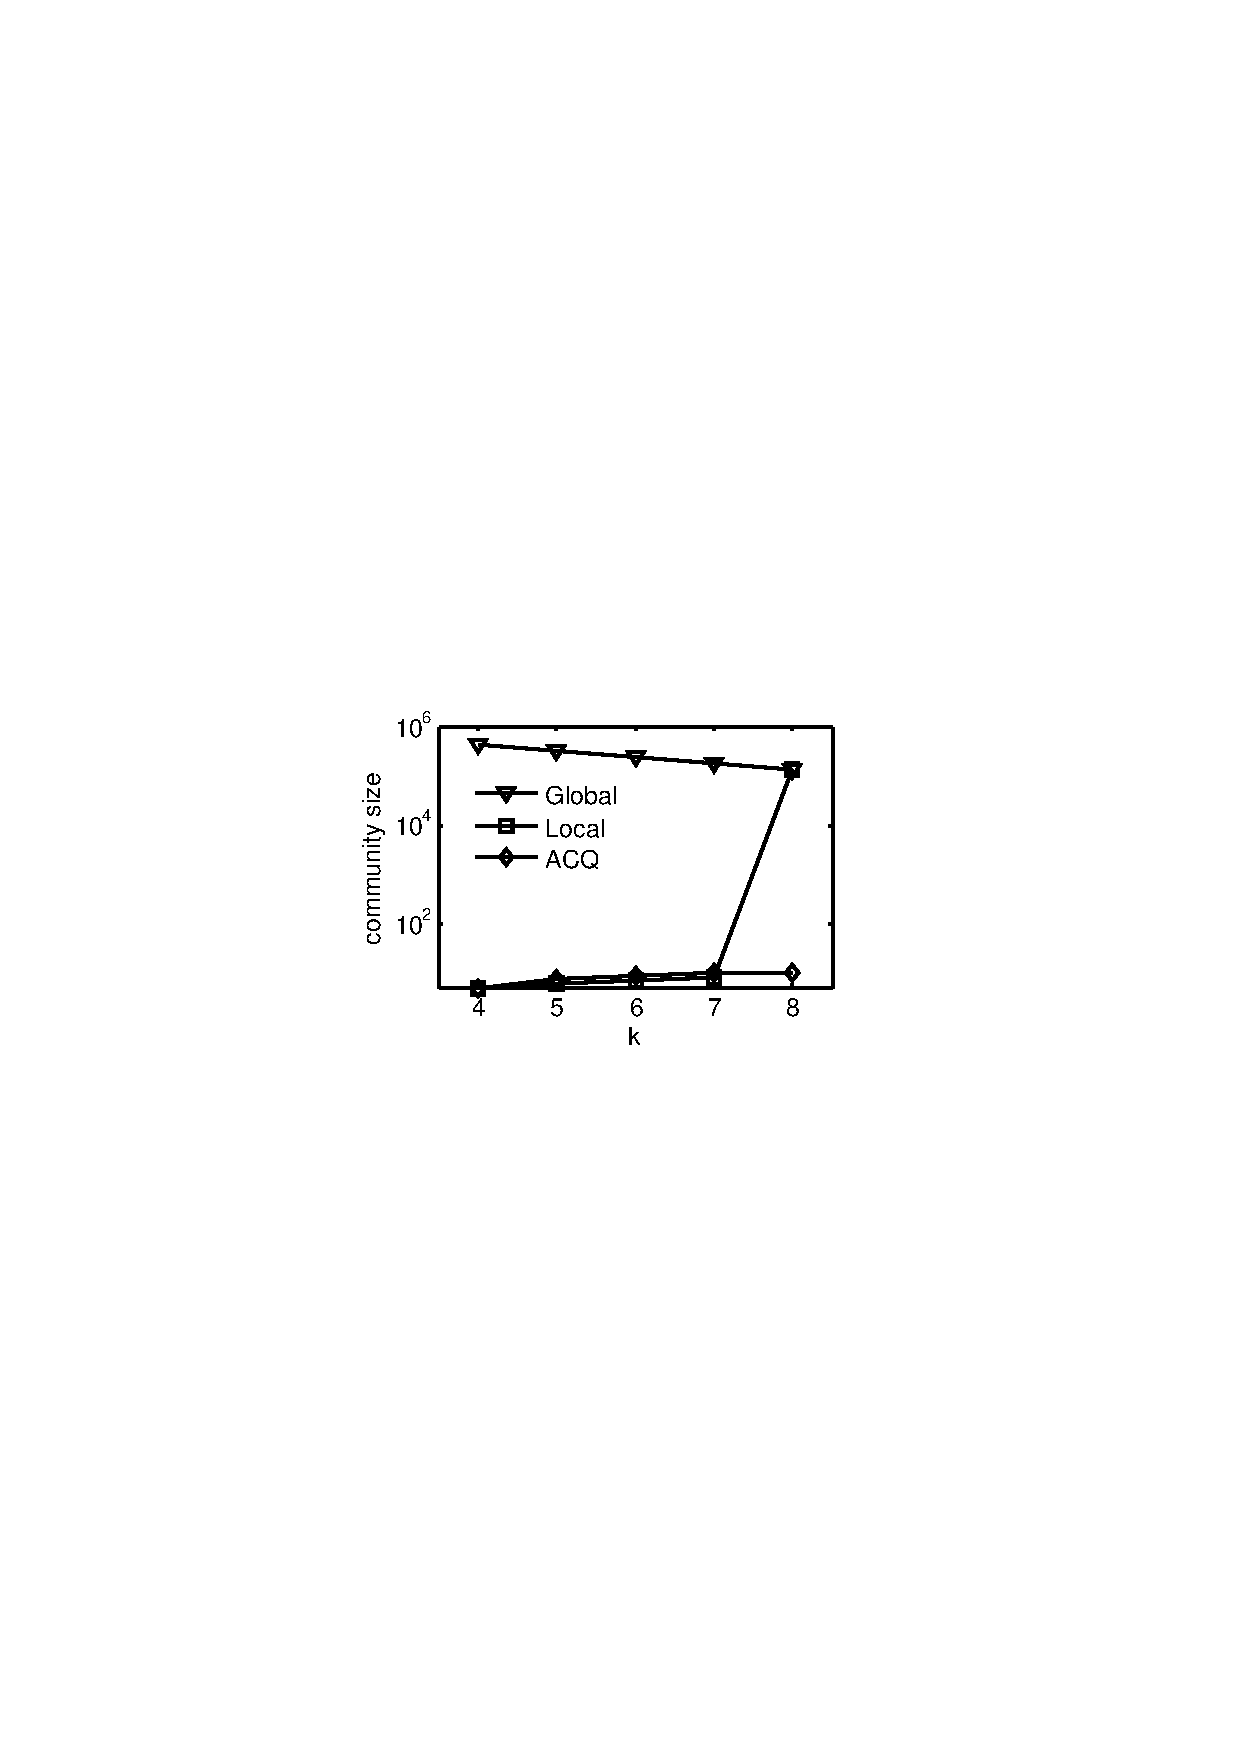
\includegraphics[width=.40\columnwidth]{figures/jim-size}
            \label{fig:jimSize}
        }
        \hspace{2ex}
        \subfigure[Jiawei Han]{
            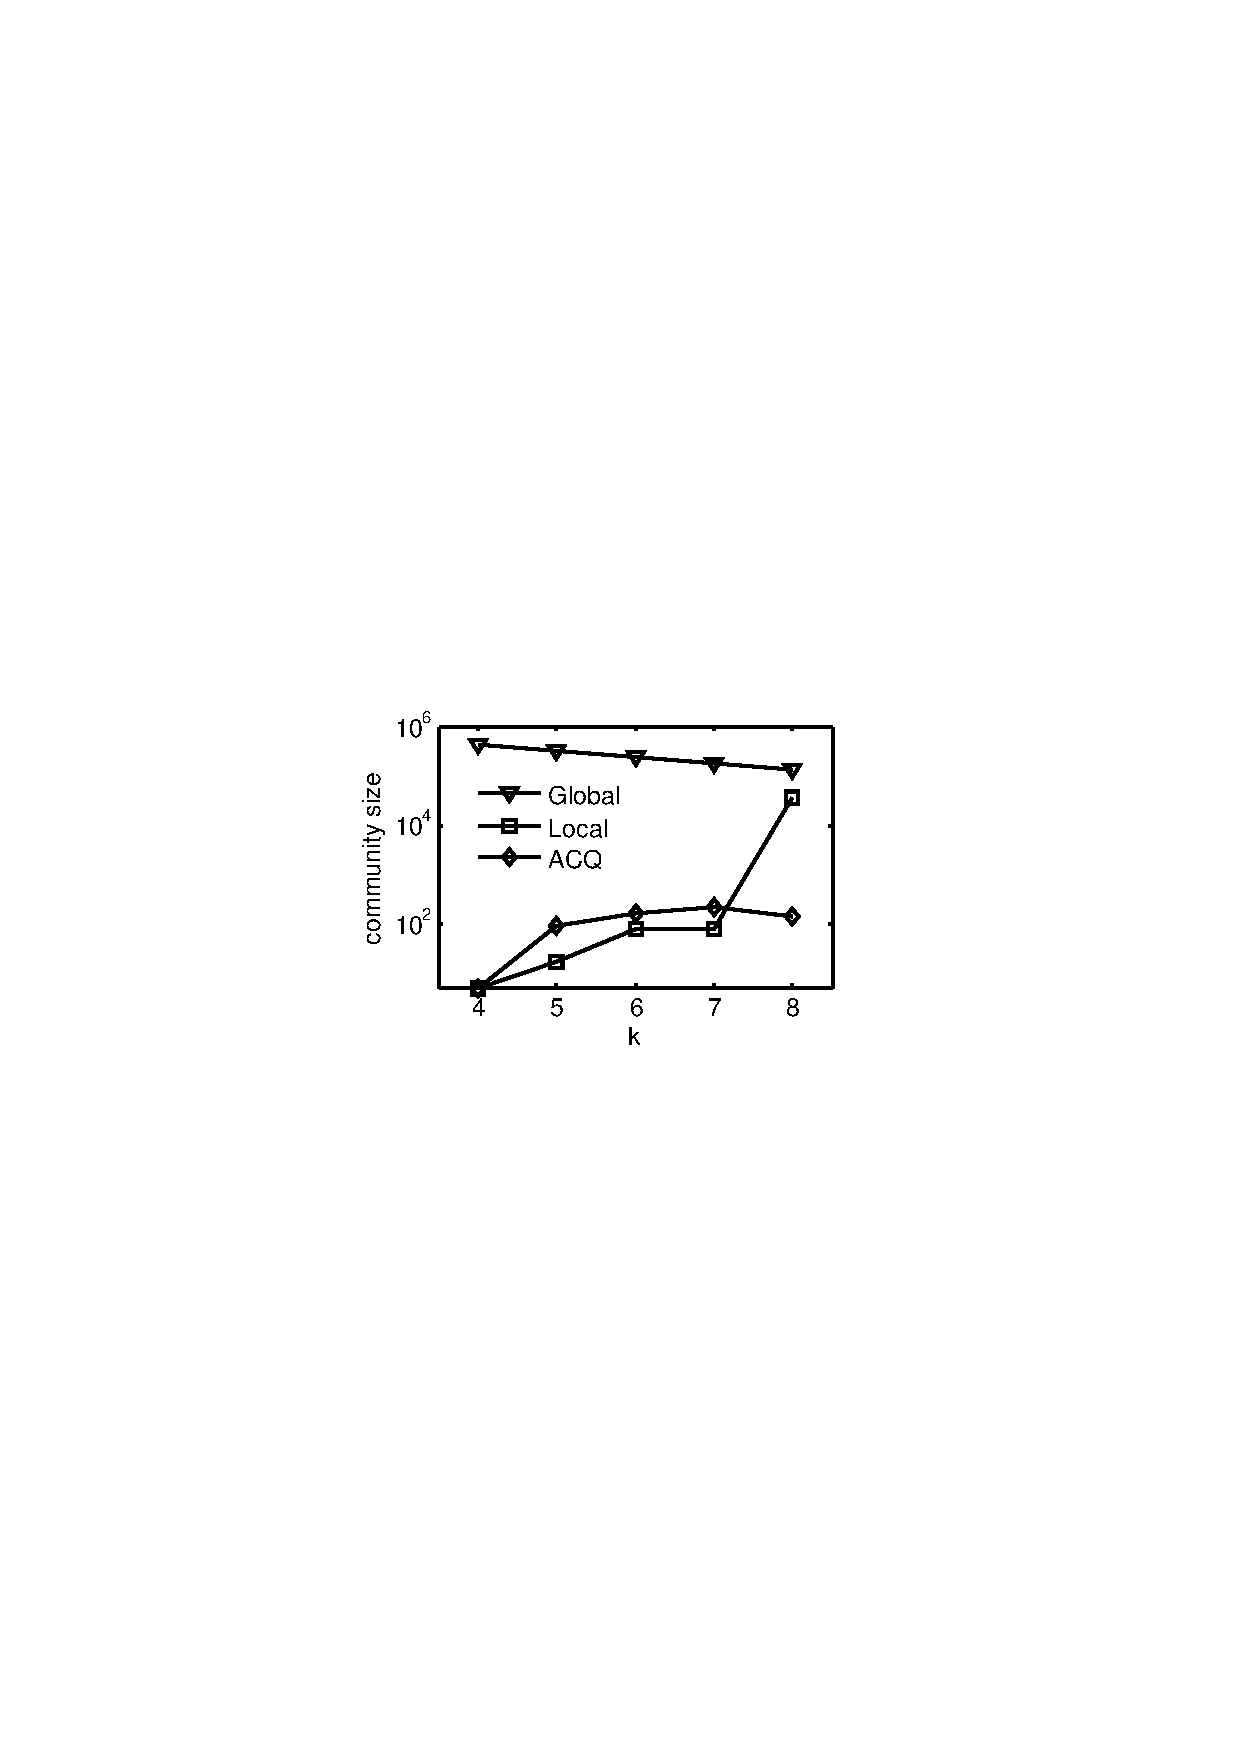
\includegraphics[width=.40\columnwidth]{figures/jiawei-size}
            \label{fig:jiaweiSize}
        }
    }
    \caption{Community size.}
    \label{fig:size}
\end{figure}


